\begin{blocksection}
\question
Registers, like the 32-bit ones in RSIC-V, are a valuable part of many circuits.  They allow the retaining of a value and constant output no matter how the input changes unless they get a signal to accept a new input.  This signal is usually the rising edge of the clock, upon which they will change their value and output to the input at the rising edge of the clock.  This means that for any input, the input must be stable for a certain amount of time both before and after the rising edge of the clock because the rising edge takes time even though it’s a very small amount.  The time before is called the setup time and the time after is called the hold time.

The circuit below is an accumulator that adds the input to the inputs previous values (i.e. after inputs 1 and 5, the accumulator should hold 6).  Both the input and the output are 8-bit unsigned integers.  The adder block (the square) adds the two inputs together and puts the result in the output wire immediately.  What is the problem with this circuit once the input changes from 0x00?

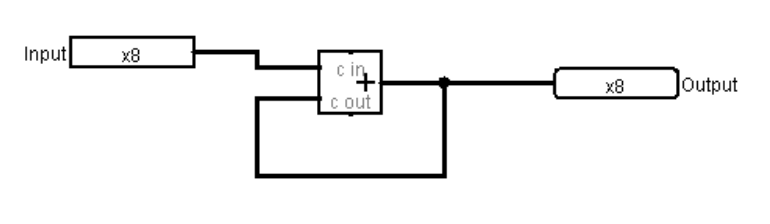
\includegraphics[width=\textwidth]{sds/registers_a}

\begin{solution}[0.5in]
The adder’s output is attached to its input without any register, so as soon as the input is taken
off 0 the adder will immediately begin to add the input to itself over and over again, making the
output 0xFF in almost no time.
\end{solution}

\end{blocksection}